\section{Manual de instalación y configuración}

En este apartado vamos a desarrollar los manuales necesarios para la instalación de la herramienta de JavaCC, el IDE de desarrollo que queramos utilizar, y el plugin de JavaCC para el IDE correspondiente.

\subsection{Instalación de JavaCC}
\label{sec:instalaciondejavacc}
Se puede utilizar JavaCC directamente desde la línea de comandos, o puede optar por utilizar un IDE, que permite desarrollar proyectos con rapidez \cite{ide} e integra varias herramientas para desarrollar proyectos de forma más eficiente y productiva.

\subsubsection{Descarga e Instalación de JavaCC desde línea de comandos}
\label{sec:descargaeinstalaciondejavaccdesdelineadecomandos}
\textbf{Descarga}

Descargue la última versión estable (al menos el código fuente y los binarios). Actualmente la versión estable más reciente es la 7.0.13, por lo que la descarga del binario se accedería a través de:

\href{https://repo1.maven.org/maven2/net/java/dev/javacc/javacc/7.0.13/javacc-7.0.13.jar}{https://repo1.maven.org/maven2/net/java/dev/javacc/javacc/7.0.13/javacc.jar}

y descargar el archivo \lstinline|javacc-7.0.13.jar|

La descarga del código fuente se realiza a través del repositorio oficial de Java CC:

\href{https://github.com/javacc/javacc/releases}{https://github.com/javacc/javacc/releases}

\textbf{Instalación}

Una vez que haya descargado los archivos, navegue hasta el directorio de descarga y descomprima el archivo fuente, creando así el llamado directorio de instalación de JavaCC:

\lstinline|unzip javacc-7.0.13.zip |

o

\lstinline|tar xvf javacc-7.0.13.tar.gz|

A continuación, mueva el archivo binario bajo el directorio de descarga en un nuevo directorio bajo el directorio de instalación y cámbiele el nombre a \lstinline|javacc-7.0.13.jar target/javacc.jar|


Posteriormente, añada el directorio del directorio de instalación de JavaCC a su archivo . Los scripts/ejecutables de invocación de JavaCC, JJTree y JJDoc residen en este directorio \lstinline|scripts/PATH|
En los sistemas basados en UNIX, es posible que los scripts no se puedan ejecutar inmediatamente. Esto se puede resolver usando el comando en el directorio \lstinline|javacc-7.0.13/|:

\lstinline|chmod +x scripts/javacc|

\subsubsection{Descarga e Instalación de JavaCC desde un IDE}

Para poder usar JavaCC en un IDE se necesita como mínimo que el IDE tenga soporte para Java, y soporte para Maven con Java. IDEs como IntelliJ o Eclipse son compatibles con JavaCC mediante la instalación de un complemento para su desarrollo.

 Descarga de IntelliJ: https://www.jetbrains.com/idea/
 
 Plugin IntelliJ JavaCC: https://plugins.jetbrains.com/plugin/11431-javacc/
 
 Descarga de Eclipse: https://www.eclipse.org/ide/
 
 Plugin Eclipse JavaCC: https://marketplace.eclipse.org/content/javacc-eclipse-plug 

Para Maven, hay que añadir la siguiente dependencia al archivo \lstinline|pom.xml|:


\lstset{inputencoding=utf8/latin1}
\lstinputlisting{code/mavendependency.xml}

En el caso de utilizar un IDE, deberá descargarse el binario, al igual que si desease desarrollar JavaCC desde la línea de comandos. Para saber el procedimiento a seguir, visite \href{sec:descargaeinstalaciondejavaccdesdelineadecomandos}{\textit{Descarga e Instalación de JavaCC desde línea de comandos}}.

\subsubsection{Configuración de JavaCC en Eclipse}

Una vez instalado JavaCC, para poder desarrollar proyectos utilizando la JavaCC en Eclipse hay que seguir los siguientes pasos:
\begin{enumerate}
    \item Crear un proyecto nuevo o elegir uno existente.
    \item Abrir las propiedades del proyecto (Alt+Enter) (\cmdkey+Enter)
    \item  Ir a \textit{JavaCC} $>$ \textit{Global Options}, y en \textit{Set the default JavaCC jar file}, poner la ruta al binario descargado anteriormente (\lstinline|javacc.jar|)
\end{enumerate}

Si mueve el binario descargado a la ruta por defecto, no es necesario realizar el paso 3. Es recomendable poner el binario en la ruta por defecto ya que, de lo contrario, para cada proyecto que quiera desarrollar va a tener que realizar este procedimiento. La ruta por defecto se indica debajo de \textit{“Set the default JavaCC jar file”} del paso 3, (default: plugin’s jar).

Si la configuración se ha realizado correctamente, a la hora de guardar los archivos JavaCC, se generarán la compilación de las clases Java correspondientes.

\begin{figure}[H]
\centering
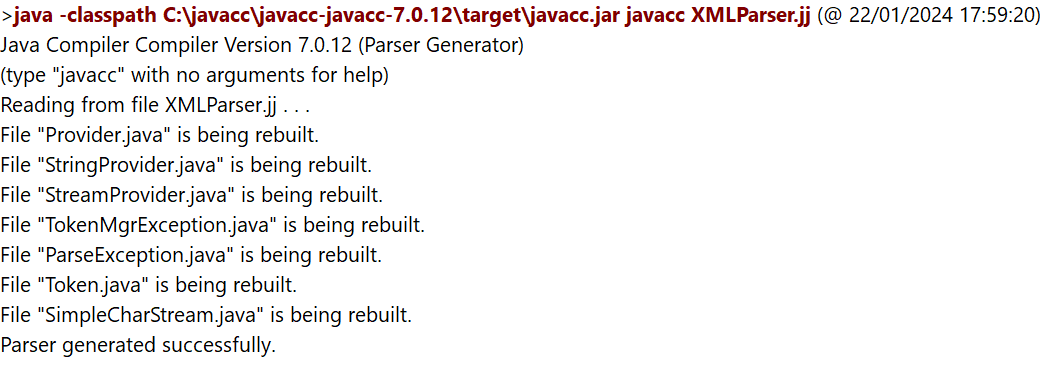
\includegraphics[width=0.9\textwidth]{imagenes/javacccompilation.png}
\caption{\label{fig:javacccompilation}Compilación de Archivos JavaCC en Eclipse}
\end{figure}
\emergencystretch=1em
\section{Símbolos de Expresiones regulares en JavaCC}
\label{sec:simbolosdeexpresionesregulares}
\lstinline[basicstyle=\large\ttfamily]|+| : El símbolo \lstinline[basicstyle=\large\ttfamily]|+| se usa para indicar que \textbf{un elemento puede aparecer una o más veces}. Por ejemplo, si tienes \lstinline[basicstyle=\large\ttfamily]|A+|, significa que se espera que haya al menos una instancia de \lstinline[basicstyle=\large\ttfamily]|A|, pero puede haber más.

\lstinline[basicstyle=\large\ttfamily]|*| : El símbolo \lstinline[basicstyle=\large\ttfamily]|*| se usa para indicar que \textbf{un elemento puede aparecer cero o más veces}. Por ejemplo, si tienes \lstinline[basicstyle=\large\ttfamily]|B*|, significa que \lstinline[basicstyle=\large\ttfamily]|B| es opcional y puede aparecer cero o más veces.

\lstinline[basicstyle=\large\ttfamily]|?| : El símbolo\lstinline[basicstyle=\large\ttfamily]|?| se usa para indicar que \textbf{un elemento puede aparecer cero o una vez}. Por ejemplo, si tienes \lstinline[basicstyle=\large\ttfamily]|C?|, significa que \lstinline[basicstyle=\large\ttfamily]|C| es opcional y puede aparecer cero o una vez.


\lstinline[basicstyle=\large\ttfamily]|~| : El símbolo \lstinline[basicstyle=\large\ttfamily]|~| se utiliza para \textbf{excluir ciertos caracteres} o elementos. Por ejemplo, \lstinline[basicstyle=\large\ttfamily]|~A| significa cualquier carácter excepto \lstinline[basicstyle=\large\ttfamily]|A|. En una expresión regular, \lstinline[basicstyle=\large\ttfamily]|~| se usa para negar un conjunto de caracteres. Por ejemplo, \lstinline[basicstyle=\large\ttfamily]|~[0-9]| significa cualquier carácter que no sea un dígito del 0 al 9.

